\documentclass[aspectratio=169]{beamer}
%% For 4:3 aspect ratio:
%% \documentclass{beamer}
\usepackage{../git-course}

\title[git-course]{Advanced Git}
\author{Chris Grandin \& Andrew Edwards}
\date{\today}

\begin{document}

\frame[plain]{
\titlepage
}

\section{Git Structure}
\frame{\frametitle{Commits and history}
  Git does not keep versions of code, it keeps \emph{commits}. The commits
  are kept track of using a hash code, using \emph{Secure Hash Algorithm 1}
  (SHA-1) which generates a hash key 40 digits long in hexadecimal. These are
  what you see on \gh\ and in various places when you use \gs.\\
  \bigskip
  Several of these commits have pointers to them which have special names:
  \bi
    \item The \textbf{HEAD} which points to the commit you are currently on
      in the \gs.
    \item The \textbf{master} which is just the default branch when you set
      up a repository on \gh.
    \item The branch names that you have in your repository.
  \ei
  Once you've cloned a \gh\ repository, the \textbf{master} points to the initial
  commit, and the \textbf{HEAD} points to the master.\\
  \bigskip
  The following slides use images from this website:
  \url{https://marklodato.github.io/visual-git-guide/index-en.html?no-svg}
}

%% Figures from : https://marklodato.github.io/visual-git-guide/index-en.html?no-svg

\frame{\frametitle{Git structure}
  \begin{columns}
    \begin{column}{0.4\linewidth}
      \bi
        \item \textcolor{green}{Green} items are commits.
        \item \textcolor{orange}{Orange} items are branches.
        \item The \textcolor{blue}{Stage} holds references to files you have
          added using \lst{git add FILE-NAME} for the next commit.
        \item The current branch is always pointed to by \textbf{HEAD}.
        \item \textbf{ed489} is the most recent commit, and it is pointed to
          by \textbf{master} and \textbf{HEAD}.
        \item \textbf{maint} is another branch, and is an ancestor of
          \textbf{master}.
      \ei
    \end{column}
    \begin{column}{0.6\linewidth}
      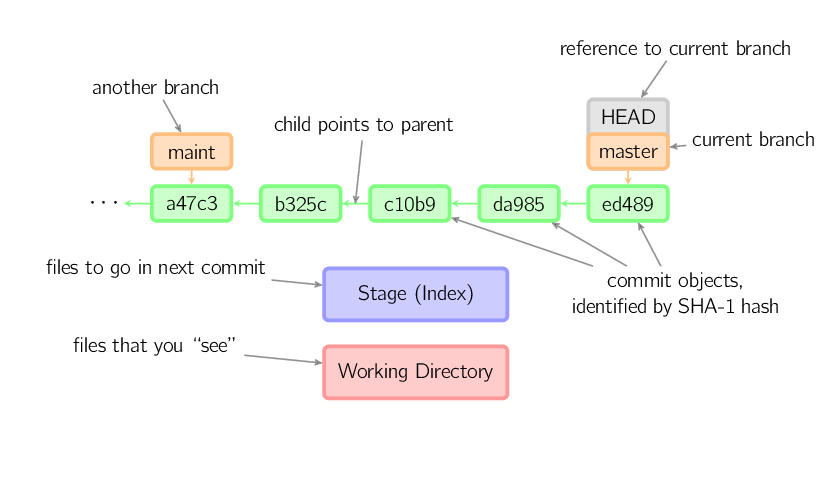
\includegraphics[
        width=\textwidth,
        height=0.8\textheight,
        keepaspectratio]
                      {figures/head-master}
    \end{column}
  \end{columns}
}

\section{Committing structure}
\frame{\frametitle{Commit on master}
  \begin{columns}
    \begin{column}{0.4\linewidth}
      \bi
        \item Any changes to files in the \textcolor{red}{Working Directory}
          will be included in the commit.
        \item Any new files you want included in the commit must be added with
          the \lst{git add FILENAME} command so that they are in the
          \textcolor{blue}{Stage} area.
        \item When you do a \lst{git commit} while in the \textbf{master}
          branch, \textbf{master} and \textbf{HEAD} are moved up one to point
          at the new commit.
      \ei
    \end{column}
    \begin{column}{0.6\linewidth}
      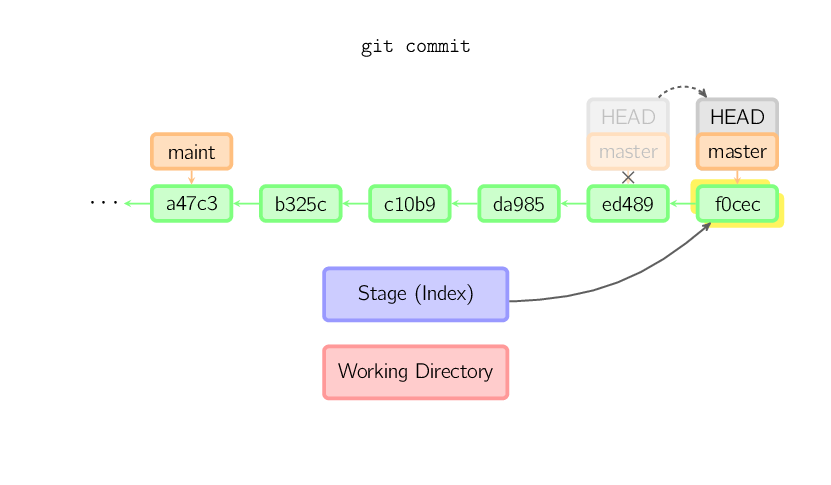
\includegraphics[
        width=\textwidth,
        height=0.8\textheight,
        keepaspectratio]
                      {figures/commit-master}
    \end{column}
  \end{columns}
}

\frame{\frametitle{Commits on another branch}
  \begin{columns}
    \begin{column}{0.4\linewidth}
      \bi
        \item If you have changed to another branch using
          \lst{git checkout maint} and then commit changes, \textbf{maint}
          and \textbf{HEAD} will be moved up to the new commit, \textbf{1800b}.
        \item \textbf{maint} is no longer an ancestor of \textbf{master}.
        \item Any files added will be a part of the \textbf{maint} branch
          and will not appear in the \textbf{master} branch.
      \ei
    \end{column}
    \begin{column}{0.6\linewidth}
      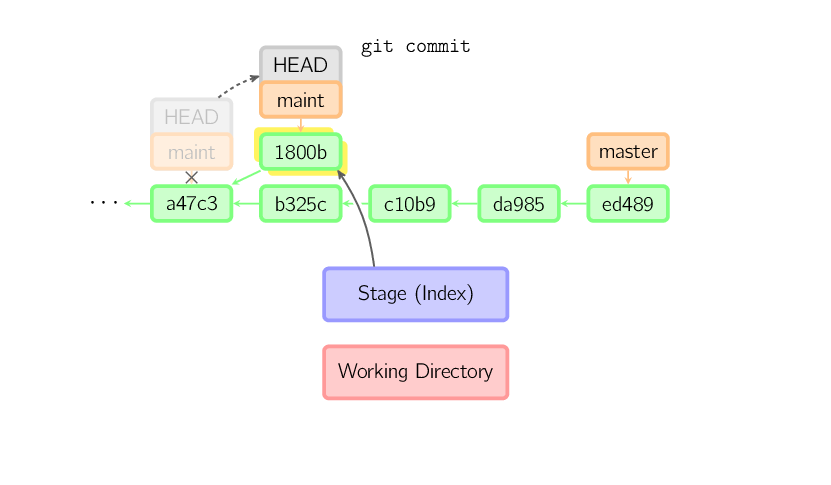
\includegraphics[
        width=\textwidth,
        height=0.8\textheight,
        keepaspectratio]
                      {figures/commit-maint}
    \end{column}
  \end{columns}
}

\frame{\frametitle{Commit amendment}
  \begin{columns}
    \begin{column}{0.4\linewidth}
      \bi
        \item If a mistake is made in the last commit, you can use
          \lst{git commit --amend}.
        \item It creates a new commit (\textbf{4ca87}) and ignores the old
          one (\textbf{ed489}).
        \item \textbf{master} and \textbf{HEAD} will be moved to the
          new commit.
        \item You can still find the old one if you want:\\
          \lst{git reflog}
      \ei
    \end{column}
    \begin{column}{0.6\linewidth}
      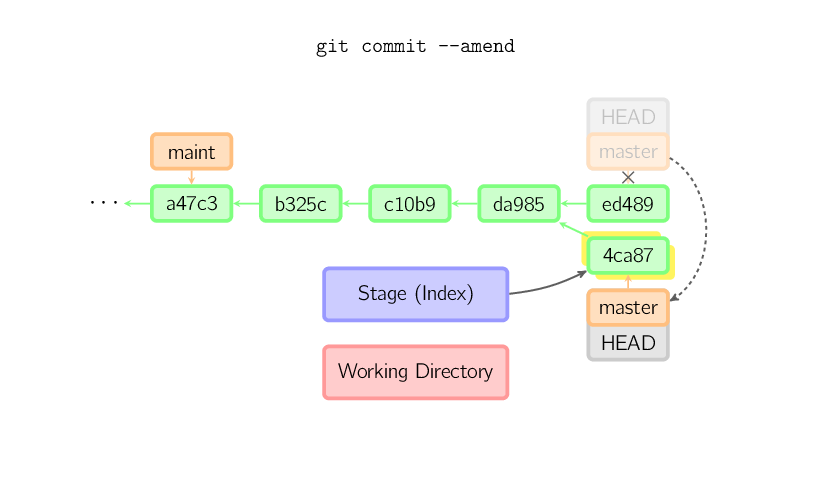
\includegraphics[
        width=\textwidth,
        height=0.8\textheight,
        keepaspectratio]
                      {figures/commit-amend}
    \end{column}
  \end{columns}
}

\section{Checking out commits}
\frame{\frametitle{Checking out any commit}
  \begin{columns}
    \begin{column}{0.4\linewidth}
      \bi
        \item You can go to any commit and see how things looked at that
          point in time. \lst{git checkout b325c} or
          \lst{git checkout master~3} will put your \textbf{HEAD} in this
          position.
        \item Your working directory will change structure to be exactly
          what is was at that commit.
        \item This is the same as changing to another branch, but there
          is no branch reference, leaving you in a \textbf{Detached Head}
          state.
      \ei
    \end{column}
    \begin{column}{0.6\linewidth}
      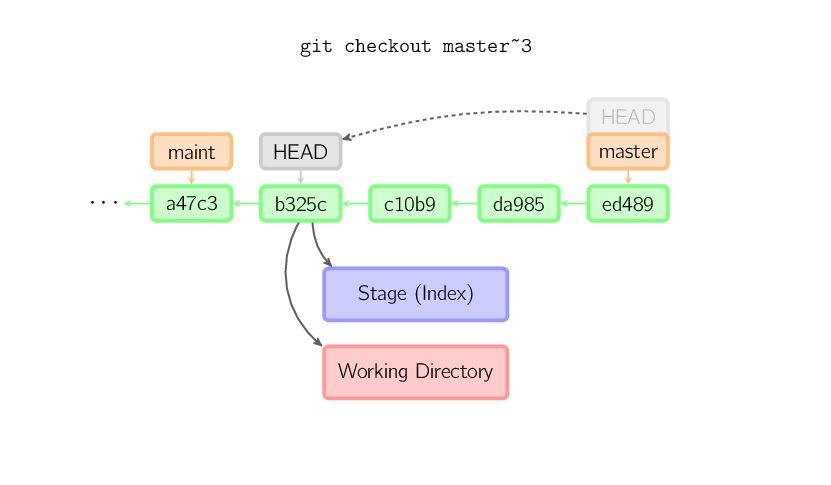
\includegraphics[
        width=\textwidth,
        height=0.8\textheight,
        keepaspectratio]
                      {figures/detached-head}
    \end{column}
  \end{columns}
}

\frame{\frametitle{Gratuitous Game of Thrones reference to a detached head}
  \centering
  \begin{figure}
    
\includegraphics[
        width=\textwidth,
        height=0.6\textheight,
        keepaspectratio]
                    {figures/ned-stark}
  \vspace{-3mm}
  \end{figure}
}

\frame{\frametitle{Committing with a detached \textbf{HEAD}}
  \begin{columns}
    \begin{column}{0.4\linewidth}
      \bi
        \item Commits work as usual, but there is no named branch so if you
          use the \lst{git checkout} command after committing in a
          detached HEAD state, you will
          \textbf{appear to lose all the work in those commits}.
        \item You can easily find them again, and go back to them by running
          \lst{git reflog}, searching for the commit message and create a
          branch there: \lst{git branch <new-branch-name> HASH}
      \ei
    \end{column}
    \begin{column}{0.6\linewidth}
      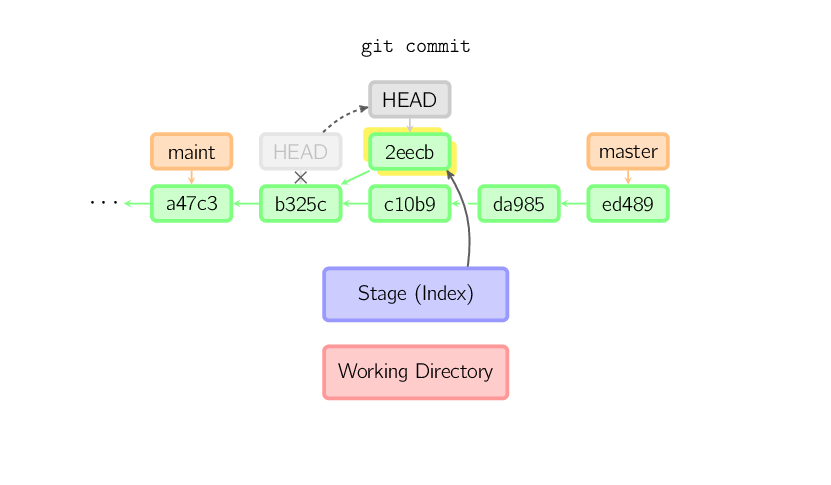
\includegraphics[
        width=\textwidth,
        height=0.8\textheight,
        keepaspectratio]
                      {figures/commit-detached}
    \end{column}
  \end{columns}
}

\frame{\frametitle{Creating a branch while in a detached \textbf{HEAD} state}
  \begin{columns}
    \begin{column}{0.4\linewidth}
      \bi
        \item Creating a branch while in a detached HEAD state will change you
          to the new branch and take you out of the detached HEAD state:\\
          \lst{git checkout -b BRANCH-NAME}\\
          or use the alias:\\
          \lst{git cb BRANCH-NAME}
      \ei
    \end{column}
    \begin{column}{0.6\linewidth}
      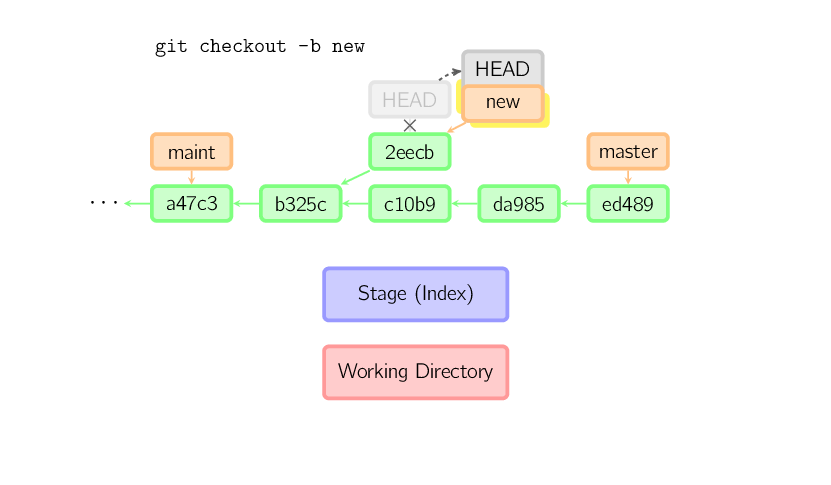
\includegraphics[
        width=\textwidth,
        height=0.8\textheight,
        keepaspectratio]
                      {figures/checkout-b-detached}
    \end{column}
  \end{columns}
}

\frame{\frametitle{If you lose your commits...}
  \begin{columns}
    \begin{column}{0.4\linewidth}
      \bi
        \item If you have made a commit in a detached HEAD state then
          checkout a different branch, you'll lose the reference
          to the commit.
        \item Find the the missing commit:\\
          \lst{git reflog}
        \item Turn your missing commit into a new branch using the \lst{HASH}
          associated with the commit:\\
          \lst{git branch BRANCH-NAME HASH}
        \item You can now checkout that branch just as any other.
      \ei
    \end{column}
    \begin{column}{0.6\linewidth}
      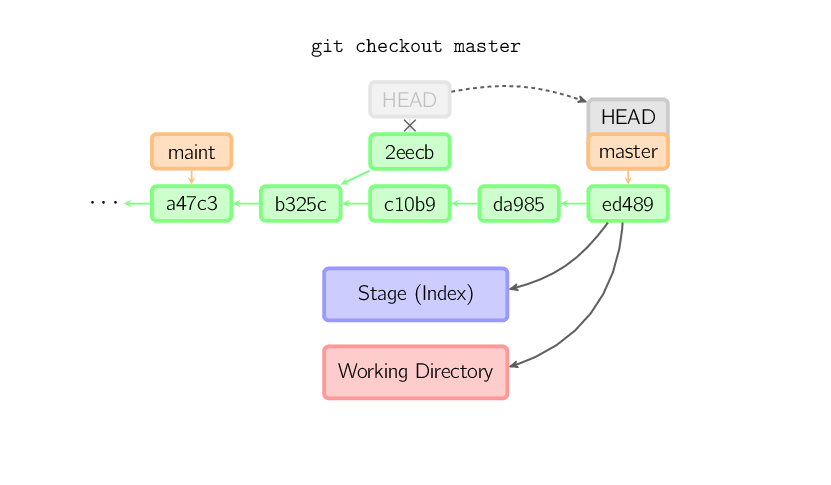
\includegraphics[
        width=\textwidth,
        height=0.8\textheight,
        keepaspectratio]
                      {figures/checkout-after-detached}
    \end{column}
  \end{columns}
}

\section{Merging}
\frame{\frametitle{Fast-forward merges}
  \begin{columns}
    \begin{column}{0.4\linewidth}
      \bi
        \item The simplest merge is the fast-forward merge.
        \item If one branch is an ancestor of the other, the reference
          is updated and nothing else needs to be done.
      \ei
    \end{column}
    \begin{column}{0.6\linewidth}
      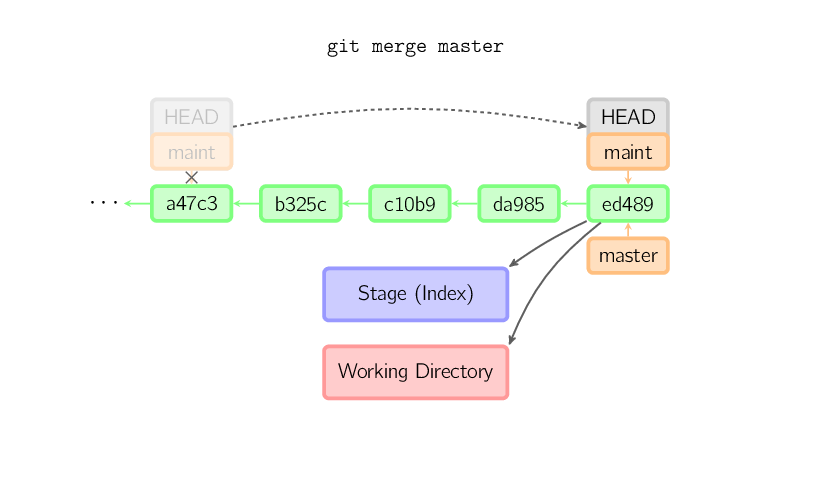
\includegraphics[
        width=\textwidth,
        height=0.8\textheight,
        keepaspectratio]
                      {figures/merge-fast-forward}
    \end{column}
  \end{columns}
}

\frame{\frametitle{Three-way merges}
  \begin{columns}
    \begin{column}{0.4\linewidth}
      \bi
        \item While in {\orange master}, the command \lst{git merge other}
          was issued.
        \item Since there have been changes in both branches, a three-way
          merge is needed.
        \item The {\orange other} (33104), {\orange master} (ed489) and their
          common ancestor (b325c) are merged.
      \ei
    \end{column}
    \begin{column}{0.6\linewidth}
      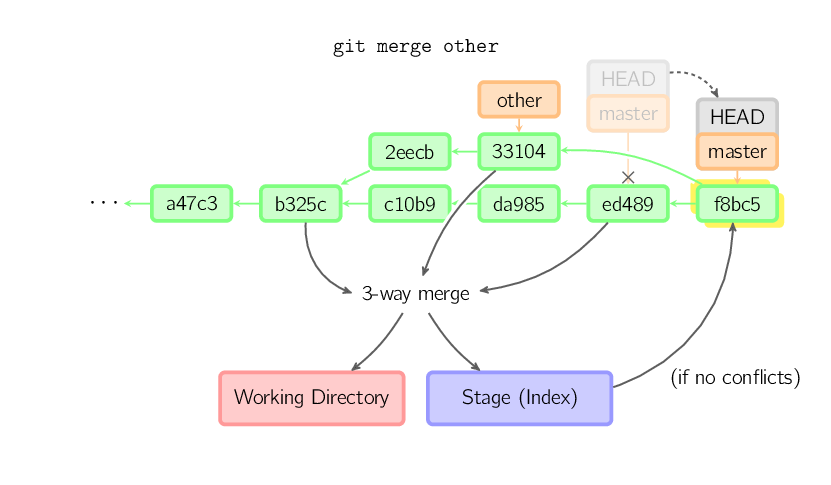
\includegraphics[
        width=\textwidth,
        height=0.8\textheight,
        keepaspectratio]
                      {figures/merge-three-way}
    \end{column}
  \end{columns}
}

\section{References}
\frame{\frametitle{References}
  \bi
    \item References are things like \textbf{HEAD}, \textbf{master},
      other branch names, and remote names.
    \item To see a list of hashes for where the \textbf{HEAD} is/was:\\
      \lst{git reflog}
    \item To see a list of hashes for the referenced objects in your local
      repository:\\
      \lst{git show-ref}\\
      This shows you which commit the objects are currently pointing to.
  \ei
}
%% To remove all unreachable (orphaned) commits:

%% git reflog expire --expire-unreachable=now --all
%% git gc --prune=now

%% The first command removes all references of unreachable commits in reflog.
%% The second commandremoves the commits themselves.

%% Only using git gc --prune=now will not work since those commits
%%  are still referenced in the reflog. Therefore, clearing the reflog is
%%  mandatory.

\section{Stashing}
\frame{\frametitle{Stashing - 1}
  You can stash more than one set of changes if you wish. To see your stack
  of available stashes:\\
  \bigskip
  \lst{git stash list}\\
  \bigskip
  The list will look something like this:\\
  \lst{stash@\{0\}: WIP on master: 46ae7a8 Merge conflict resolved.}\\
  \lst{stash@\{1\}: WIP on master: fe35a9b Minor change to Readme.}\\
  where each commit the stash was based on is listed. You can apply any
  of these by using the syntax:\\
  \bigskip
  \lst{git stash apply "stash@\{N\}"}\\
  \bigskip
  where \lst{N} is one of the numbers shown. If you don't specify a stash, the
  most recent one (\lst{stash@\{0\}}) is used:\\
  \bigskip
  \lst{git stash apply}
}

\frame{\frametitle{Stashing - 2}
  If you use the \lst{git stash apply} command, the commit which is
  applied will remain in the stash list. To apply the stash and also remove
  it from the stash list:\\
  \bigskip
  \lst{git stash pop}\\
  or\\
  \lst{git stash pop "stash@\{N\}"}\\
  \bigskip
  To remove stash commit N without applying it:\\
  \bigskip
  \lst{git stash drop "stash@\{N\}"}\\
  \bigskip
  To remove the top (most recent) stash commit without applying it:\\
  \bigskip
  \lst{git stash drop}\\
  \bigskip
  If you are cleaning up your repository, you can remove everything in the
  stash list:\\
  \bigskip
  \lst{git stash clear}
}

\frame{\frametitle{\lst{git merge} gone wrong - which is the HEAD?}
  \centering
  \begin{figure}
    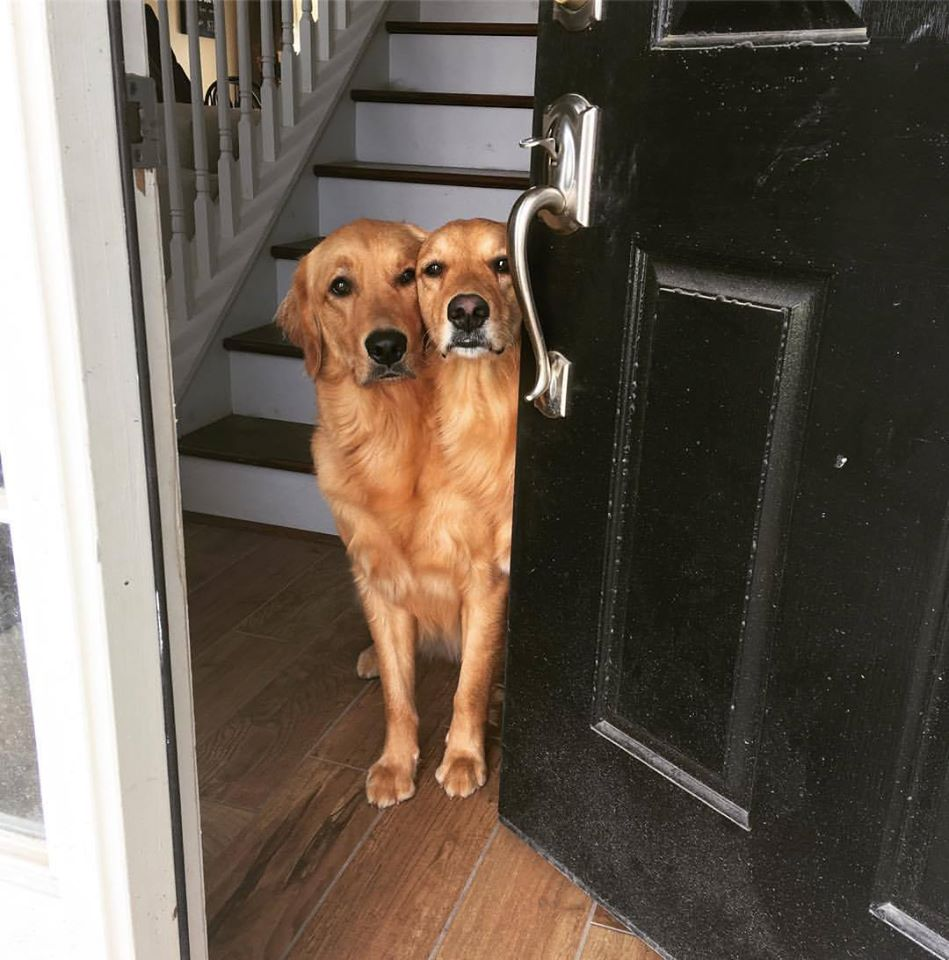
\includegraphics[
        width=\textwidth,
        height=0.8\textheight,
        keepaspectratio]
                    {figures/git-merge-failed-dogs}
  \vspace{-3mm}
  \caption{\tiny\url{https://www.reddit.com/user/NegativePitch}}
  \end{figure}
}

%% Dog pic:
%% https://www.reddit.com/user/NegativePitch
%% http://i.imgur.com/zxm6UAh.jpg

\section{Workflow}

\frame{\frametitle{Git Workflow}
  There are two ways to work using Git and \gh:

  \bn
    \item A project where collaborators work closely together and each have
      a copy of the repository, none of which are the 'master copy'.
      \bi
        \item Fork a copy from the initial creator's repository.
        \item Merge other people's remote repositories into yours using \gs.
      \ei
    This is what we always do, as we are mostly working on assessments
    or other smallish projects closely with collaborators.
    \item A project where people contribute to a main repository that is
      considered the 'master copy'.
      \bi
        \item Don't fork, instead clone directly from the creator's repository.
        \item Send a \emph{Pull request} to the creator on the \gh\ site. They
          accept your pull request and your code is merged into the 'master
          copy'.
      \ei
       Andy tried this one with a student and we kept getting in a mess.
       This is more suited to large public projects.
  \en
}

\end{document}
